\documentclass{article} %this is an article
\usepackage[lmargin=.75in,rmargin=.75in,tmargin=1.in,bmargin=1in]{geometry} % setting margins
%\usepackage{tree-dvips}
\usepackage{tikz}  %makes crazy graphs
\usepackage{enumitem}
% \usetikzlibrary{snakes}
%\usepackage[flushleft]{threeparttable} %% makes notes for tables that wraps around width of table
%\usepackage{chronology}
\usepackage[round]{natbib}  %% beatiful bibliography
%\usepackage{wrapfig}
%\usepackage{longtable} %%multipage table
%\usepackage{qtree}
\usepackage{verbatim} %all kinds of shit
\usepackage{graphicx} %beautiful figures
%\usepackage{graphics}
%\usepackage{color}
%\usepackage{caption}
\usepackage{subcaption} %subcaption on the the subfigures
%\usepackage{multirow}
%\usepackage{sidecap}
%\usepackage{epstopdf}
\usepackage{amssymb} %beautiful math
\usepackage{amsmath,amssymb,amsfonts,amsthm,array} %beautiful math
\usepackage{amsthm}  %beautiful math
\usepackage{pgfplots}  %Normal distribution figure
\usepackage[colorlinks=true,linkcolor=red, citecolor=red]{hyperref} %sets my preferences for cross reference



\begin{document}
\begin{center}
  \textbf{Joao Rodrigues} \\
  \textbf{Economics 8185 - Computational Methods} \\
  \textbf{Homework 3a - Krusell \& Smith (1998)} \\
  \textbf{Economics Department}
\end{center}
\section*{Model details}
In the Krusell \& Smith (1998) economy, there is a continuum of agents who consume $c_t$, save in $a_{t+1}$, value leisure $l_t$ and supply his/her non-leisure time to labor ($1-l_{t}$). The individual problem can be defined for an individual who takes the interest rate $r$ and wage rate $w$ as given according to:
\begin{align*}
  v(k,\epsilon;K,L,z) & = \max_{\{a'_t, l_t\}}  \quad  U(c,l) + \beta E[v(k',\epsilon';K',L',z')]   \\
  st:  & \quad c_t + a_{t+1} = (1+r(K,L,z))a_{t} + (1.0-l)w(K,L,z)\epsilon\\
       & \quad K' = a_{K,0} + a_{K,1}K\quad if \quad z = z_g \\
       & \quad K' = b_{K,0} + b_{K,1}K\quad if \quad z = z_b \\ 
       & \quad L = a_{L,0} + a_{L,1}K\quad if \quad z = z_g \\
       & \quad L = b_{L,0} + b_{L,1}K\quad if \quad z = z_b \\ 
           & \quad a_{t+1} \geq 0
\end{align*}
There is a representative firm who demands labor and capital while also taking prices as given. The firm's technology is Cobb-Douglas and it maximizes profit. Accordingly, prices must satisfy: 
%%%
$$r = \alpha (L/K)^{1-\alpha} - \delta \Rightarrow w = (1-\alpha)(L/K)^{\alpha} $$
%%%
We'll construct a rational expectations equilibrium where aggregate savings and labor supply from consumers are used in production by the representative firm. There are prices $r,w$ that rationalize these allocations. These prices are not observable but agents have a belief over the evolutoin of aggregates (which determines these prices). In a rational expectations equilibrium, we need to find the law of motion that closely rationalizes individual allocations so that agents predict prices sufficiently well. 
\section*{Computation}
I start the algorithm with a guess for the law of motion for $K'$ an $L$
\begin{enumerate}
\item solve the individual problem given these laws of motion
\item compute the transitional distribution based on individual policies.
\item simulate a long time series clearing both capital (trivially) and labor markets in each period in the simulation and recording aggregate capital and labor 
\item Find coefficients $a_{K,0},a_{K,1},b_{K,0},b_{K,1},a_{L,0},a_{L,1},b_{L,0},b_{L,1}$ by estimating 4 regressions for the 4 laws of motion based on the times series for K and L 
\item If laws of motion converge, stop otherwise, update according to
  $$ LoM = \alpha LoMnew + (1-\alpha) LoMold  $$
  and go back to 1
\end{enumerate}
%%%%
I solved both the exogenous and endogenous labor cases. In the exogenous labor case, the law of motion for capital converges in less than a minute but improvements in my code and reduction of unecessarily large grid could reduce this time even further. The endogenous labor case once again adds new complexities. We have to clear labor markets in each time period in the simulation and I do this via Newton's algorithm in the same way it was implemented in the Aiyagari (1994) case. Hence, in the similation, capital decisions determine the evolution of capital holdings, and this evolution relies on individual policies derived from agents forecasting prices according to their beliefs about them. Although capital markets clear trivially, agents' labor decisions will not aggregate exactly to the labor demand, so any deviation from market clearing is due to a miscalculation based on the agent's erroneous belief about $L$. But markets need to clear, and as agents forecast prices better and better, this discrepancy will only get smaller and smaller. So in each time period in the simulation (after solving individual policies based on preceived laws of motion), we need to build a time series by updating aggregate capital next period and aggregate labor this period. In other words, fix a solution to individual problem and in each period:
\begin{enumerate}
\item compute aggregate capital tomorrow based on transitional distribution
\item use L as a parameter in prices, update labor decisions and aggregte them until $\sum_i\lambda(i,\epsilon)*(1-l(k)) = L$
  \end{enumerate}
As far as technology and preference parameters, we used the following utility:
$$ u(c,l) = \frac{[c^{\theta}(1-l)^{1-\theta}]^{1-\sigma}-1}{1-\sigma} $$
with $\sigma=1$ and $\theta=1/2.9$. As far as production, we have as before $\alpha=0.36$ and $\delta=0.025$ 
%%%%%%%
%%%%%%%
\section*{Results}
\subsection*{Exogenous labor}
In the exogenous labor case, I don't need to clear labor markets and capital markets clear trivially since agents enter a period with $k$ and each choose $k'$ while $l$ is determined along with $k'$. Below are my results for the exogenous case. 
\begin{table}[h!]
  \centering
\begin{tabular}{c c c}
  $K' = 0.094 (0.095) + 0.963 (0.962)*K$ & $z = z_g$ & $R^2 = 0.999998$ \\
  $K' = 0.084 (0.085) + 0.965 (0.965)*K$ & $z = z_b$ & $R^2 = 0.999998$
\end{tabular}
\caption{Exogenous labor law of motion (KS results in parenthesis)}
\end{table}
%%%%%%%%%%%%%%%%%%%
Unlike my solution for Aiyagari (1994), I tried to replicate Krusell \& Smith results by using exactly the parameters used in the paper. I used different methods to solve for the policy (Finite element method as in Aiyagari) and the distribution (I used Young (2010) while they used simulation). Below, I show the distribution of assets at the last period of the simulation when the laws of motion converge, the law of motion compared to the implied law of motion, and the individual policies.
\begin{figure}[h!]
  \centering
  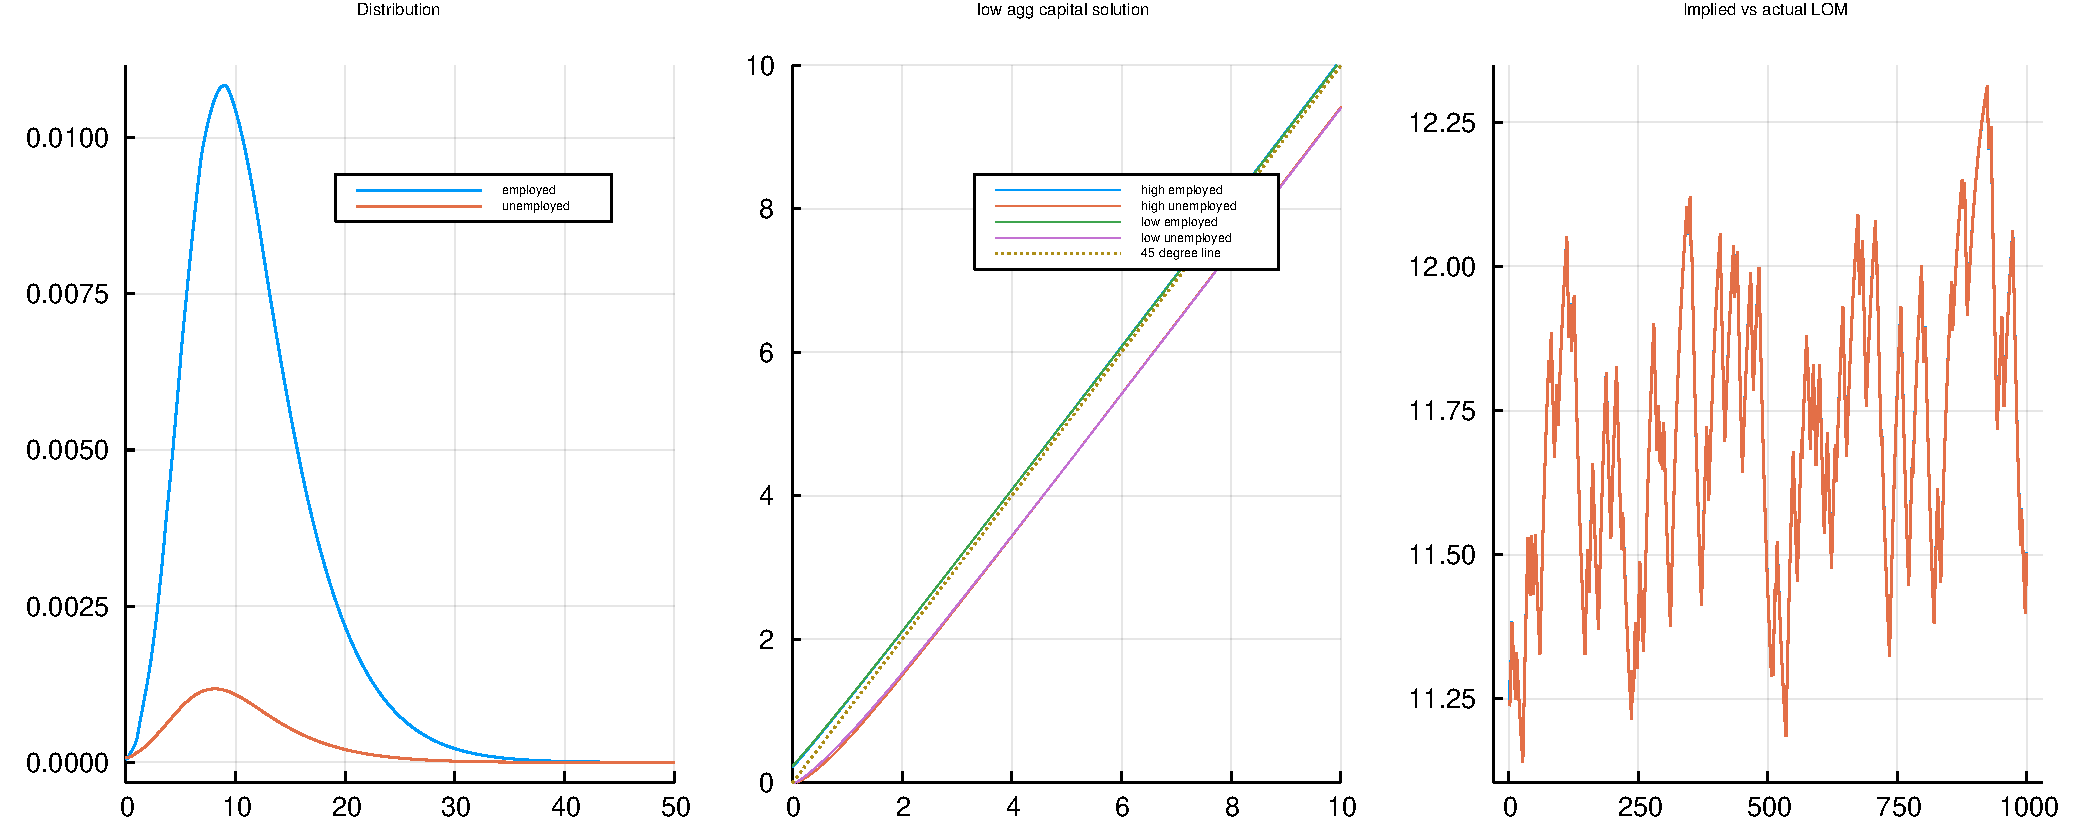
\includegraphics[width = 0.8\textwidth]{../KS_Inelastic/exolaborks.pdf}
    \caption{$u(c)=\log(c),\; \beta = 0.99,\; \alpha=0.36,\; \delta =0.025$}
  \end{figure}
\subsection*{Endogenous labor}
With endogenous labor, the the problem became very sensitive to my guess for the law of motion. Starting with a bad guess for the law of motion would bring the law of motion way off so that the individual problem would no longer converge. I started by postulating a law of motion that looked a lot like the one in the paper to see if my algorithm solved. I then moved away from it t see if It would converge to the same parameters. In fact, my estimation came very close to the results in the paper. My law of motion for capital matched it to the 3rd decimal while my law of motion for labor oscillated a bit but still came very close (not as close understanbly since the $R^2$ is lower). Below are my estimates:
\begin{table}[h!]
  \centering
\begin{tabular}{c c c}
  $K' = 0.122 (0.123) + 0.951 (0.951)*K$ & $z = z_g$ & $R^2 = 0.999997$ \\
  $K' = 0.111 (0.114) + 0.953 (0.953)*K$ & $z = z_b$ & $R^2 = 0.999995$ \\
  $L = -0.554 (-0.544) - 0.250 (-0.252)*K$ & $z = z_g$ & $R^2 = 0.997$ \\
  $L = -0.616 (-0.592) - 0.247(-0.255)*K$ & $z = z_b$ & $R^2 = 0.995$ \\
\end{tabular}
\caption{Exogenous labor law of motion (KS results in parenthesis)}
\end{table}
The results show that we get very close to the results reported in the paper. Further, any discrepancy may be due to different methods used in both the computation of individual policies and transitional distributions. As in Ayiagari, we get a less skewed distribution of assets with endogenous labor as agents can adjust their hours as well as accumulate/decumulate assets. 
\begin{figure}[h!]
  \centering
  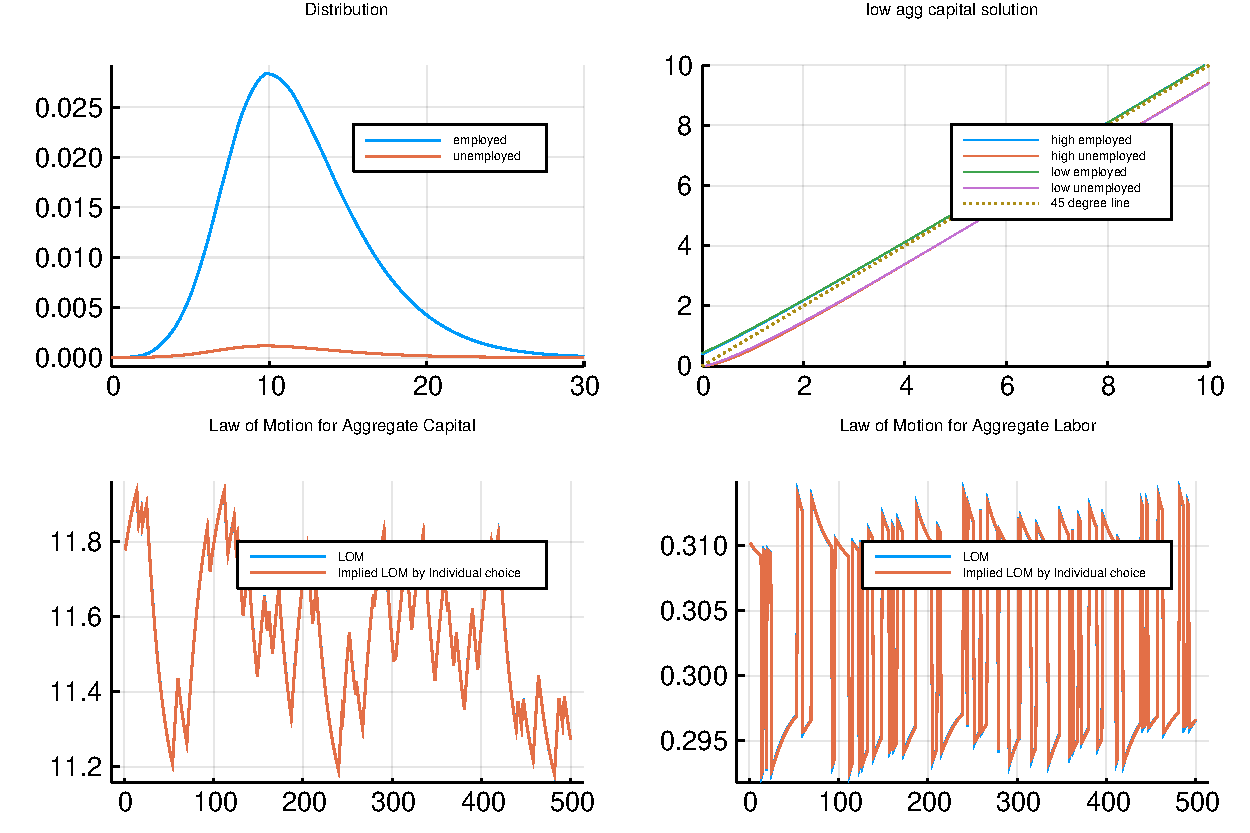
\includegraphics[width = 0.8\textwidth]{../KS_Elastic/endlaborks.pdf}
    \caption{$u(c)=\log(c),\; \beta = 0.99,\; \alpha=0.36,\; \delta =0.025$}
  \end{figure}
Figure two displays similar figure to the exogenous labor case. We can see that agents do a very good job at predicting the aggregate capital and labor. It can also be seen that they do a worse job at predicting aggregate labor (more of the blue can be seen) but still very good. 
\end{document}
